\documentclass[a4paper, 11pt, twoside]{report} %twoside
\title{Programación y Código Libre}
\author{David Davó \and Julio}
\date{\today{}}

%%Packages
\usepackage[utf8]{inputenc} %Para saber el encoding del archivo
\usepackage[no-math]{fontspec} %Para usar fuentes del sistema

\usepackage[xindy, nomain, acronym, nonumberlist, nopostdot]{glossaries}

\usepackage{graphicx} %Para insertar gráficos
\usepackage{float} %PAra posicionar bien los gráficos
\usepackage{unicode-math} %Para símbolos matemagicos
%\setmathfont{Latin Modern Math}
\setmathfont{Asana-Math.otf}
\usepackage[type={CC}, modifier={by-sa}, version={4.0}]{doclicense} %Muestra la licencia
\usepackage[usenames,svgnames,table]{xcolor} %Para darle color
\usepackage{dirtytalk} %Usado para citar
\usepackage{csquotes} %lo mismo qu eel anterior pero con estilo
\usepackage[spanish]{babel} %Hace que el idioma de los defaults esté en Español
\usepackage{fancyhdr} %Para poner encabezados y pies de página
%De la bibliografía y las citas.
\usepackage[
backend=biber
]{biblatex}
\addbibresource{Bibl.bib}

%Decoraciones y formato del texto
\usepackage[left=2.75cm, right=2cm, top=3cm, bottom=3cm]{geometry}
\usepackage{multirow}

\setmainfont{Arial}
\setmonofont{Inconsolata}
\fontsize{11}{14}
%Pies de pagina y eso
\pagestyle{fancy}
\fancyhf{}
\fancyhead[LE, RO]{David Davó}
\fancyhead[RE, LO]{Programación y Código Libre}
\fancyfoot[LE, RO]{\thepage}
\fancyfoot[C]{\leftmark}

\makeglossaries
\newglossaryentry{Libr}
{
	name=Librería,
	description={En informática, una librería o biblioteca es un conjunto de recursos y fucniones diseñadas para ser usadas por otros programas. Incluyen plantillas, funciones y clases, subrutinas, código escrito, variables predefinidas...},
	plural=librerías,
}
\newglossaryentry{datos}{
	name=Datos,
	description={Secuencia binaria de unos y ceros que contiene información codificada},
	plural=Datos, 
}
\newacronym{gnu}{GNU}{\textit{GNU's Not Unix} (GNU no es Unix)}
\newglossaryentry{Linux}
{
  name=Linux,
  description={is a generic term referring to the family of Unix-like
               computer operating systems that use the Linux kernel},
  plural=Linuces
}
\newglossaryentry{conmutacion de paquetes}{
	name={Conmutación de paquetes},
	description={Método para enviar datos por una red de computadoras. Se divide el paquete en dos partes, una con información de control que leen los nodos para enviar el paquete a su destino y los datos a enviar},
}
\newacronym{osi}{OSI}{\textit{Open Systems Interconnection} (Interconexión de Sistemas Abiertos)}
\newglossaryentry{gls-ISO}{
	name={\textit{International Organization for Standardization}},
	description={Organización Internacional de Normalización. Compuesta de varias organizaciones nacionales se encarga de la creación de estándares internacionales desde 1947.},
}
\newacronym[see={[Glossary:]{gls-ISO}}]{iso}{ISO}{\textit{International Organization for Standardization}\glsadd{gls-ISO}}
\newglossaryentry{capas de abstraccion}{
	name={capas de abstracción},
	description={Método de ocultar detalles de implementación de un set de funcionalidades},
}
\newacronym{IEEE}{IEEE}{Instituto de Ingeniería Eléctrica y Electrónica}
\newglossaryentry{topologia de red}{
	name={topología de red},
	description={Configuración espacial o física de la red. (Ver \ref{topdred} pág.\pageref{topdred})},
	plural={topologías de red},
	see={topologia}
}
\newglossaryentry{topologia}{
	name={topología},
	description={``Rama de las matemáticas que trata especialmente de la continuidad y de otros conceptos más generales originados de ella, como las propiedades de las figuras con independencia de su tamaño o forma." \cite{rae}[Topología]},
	plural={topologías},
}
\newglossaryentry{hardware}{
	name={hardware},
	description={Conjunto de elementos físicos o materiales que constituyen un sistema informático.},
}
\newacronym{MAC}{MAC}{\textit{Media Access Control}, Control de Acceso al Medio}
\newacronym{ADSL}{ADSL}{\textit{Asymmetric Digital Subscriber Line} [Línea de Abonado Digital Asimétrica]}
\newacronym{LAN}{LAN}{\textit{Local Area Network} [Red de Área Local]}
\newacronym{FTTH}{FTTH}{\textit{Fiber To The Home} [Fibra hasta el hogar]}
\newacronym[see={[Glossary:]{gls-FTTx}}]{FTTx}{FTTx}{\textit{Fiber to the X \glsadd{gls-FTTx}}}
\newglossaryentry{gls-FTTx}{
	name={FTTx},
	description={Término que agrupa las distintas configuraciones de acometida de la fibra óptica.},
}
\newglossaryentry{bit}{
	name={bit},
	description={\textit{\textbf{Bi}nary digi\textbf{t}, o dígito binario. Cada dígito del sistema de numeración binario}},
	plural={bits}
}
\newacronym{POP3}{POP3}{\textit{Post Office Protocol}, Protocolo de Oficina Postal}
\newacronym{url}{URL}{\textit{Uniform Resource Identifier}, Identificador de Recursos Uniforme}
\newglossaryentry{cache}{
	name={caché},
	description={Almacenamiento temporal de datos con el objetivo de reducir el retardo, la carga de los servidores y el ancho de banda consumido},
}
\newglossaryentry{programacion imperativa}{
	name={programación imperativa},
	description={Las órdenes del programa cambian el estado de este mismo. Por ejemplo, una variable no tiene por que ser declarada con antelación y su valor es modificable. Es la que usa el código máquina de los ordenadores},
}
\newglossaryentry{botnet}{
	name={botnet},
	description={Grupo de ordenadores coordinados conectados a un maestro mediante un virus. Gracias a este virus se pueden realizar tareas masivas como el envío de SPAM o ataques DDoS},
}
\newglossaryentry{bug}{
	name={bug},
	plural={bugs},
	description={Error en un programa informático.},
}
\newglossaryentry{repositorio}{
	name={repositorio},
	plural={repositorios},
	description={Servidor donde se alojan ficheros o archivos para su descarga},
}
\newglossaryentry{dependencia}{
	plural={dependencias},
	name={dependencia},
	description={De un programa, otro tipo de software necesario para que éste funcione}
}
\newacronym{FSF}{FSF}{\textit{Free Software Foundation}, Fundación del Software Libre}
\newacronym{IDE}{IDE}{Entorno de Desarrollo Integrado, \textit{Integrated Development Enviroment}}
\newacronym{GUI}{GUI}{Interfaz Gráfica de Usuario, \textit{Graphic User Interface})}

%Document
\begin{document}

\begin{titlepage}
{\Large\maketitle}
\pagenumbering{gobble}
\end{titlepage}
\clearpage

\tableofcontents
\newpage{}
\pagenumbering{arabic}

\chapter{Programación y código libre}

\subsection*{Propuesta}
El objetivo es el desarrollo de un software programado en Python de código libre con el que los alumnos puedan aprender tanto sobre redes como de programación en Python.

\section{Herramientas}
El programa ha sido creado con herramientas de software libre. Según la Free Software Foundation
\say{«Software libre» es el software que respeta la libertad de los usuarios y la comunidad. A grandes rasgos, significa que los usuarios tienen la libertad de ejecutar, copiar, distribuir, estudiar, modificar y mejorar el software. Es decir, el «software libre» es una cuestión de libertad, no de precio. Para entender el concepto, piense en «libre» como en «libre expresión», no como en «barra libre». En inglés a veces decimos «libre software», en lugar de «free software», para mostrar que no queremos decir que es gratuito.}
--\cite{FSF-Ph}

Todas las herramientas citadas a continuación, son o están basadas en Software Libre.

\subsection{GNU/Linux}
GNU/Linux, también llamado incorrectamente sólo Linux, es una manera de llamar al Sistema Operativo (OS) combinación del kernel Linux (Basado en Unix) y el OS \gls{gnu}, ambos software son libres y de código abierto. Normalmente Linux se distribuye en distribuciones o 'distros', las cuales contienen paquetes de software preinstalados, dependiendo del grupo de usuarios al que este dirigida.

\subsubsection*{Distros}

\subsection{Git y Github}
Git es un software diseñado por Linus Torvalds con el que puedes crear un Sistema de Control de Versiones o VCS (\textit{Version Control System}). Este programa te permite de forma sencilla volver a una versión o \textit{commit} anterior del programa, así como enviarlas a un repositorio remoto e incluso publicarlas en línea. Su punto fuerte son las \textit{branches} o ``ramificaciones" del código, haciendo que la rama \textit{master} (principal) siempre pueda ser usada. Para ello creamos una nueva rama para cada nueva funcionalidad del programa.

%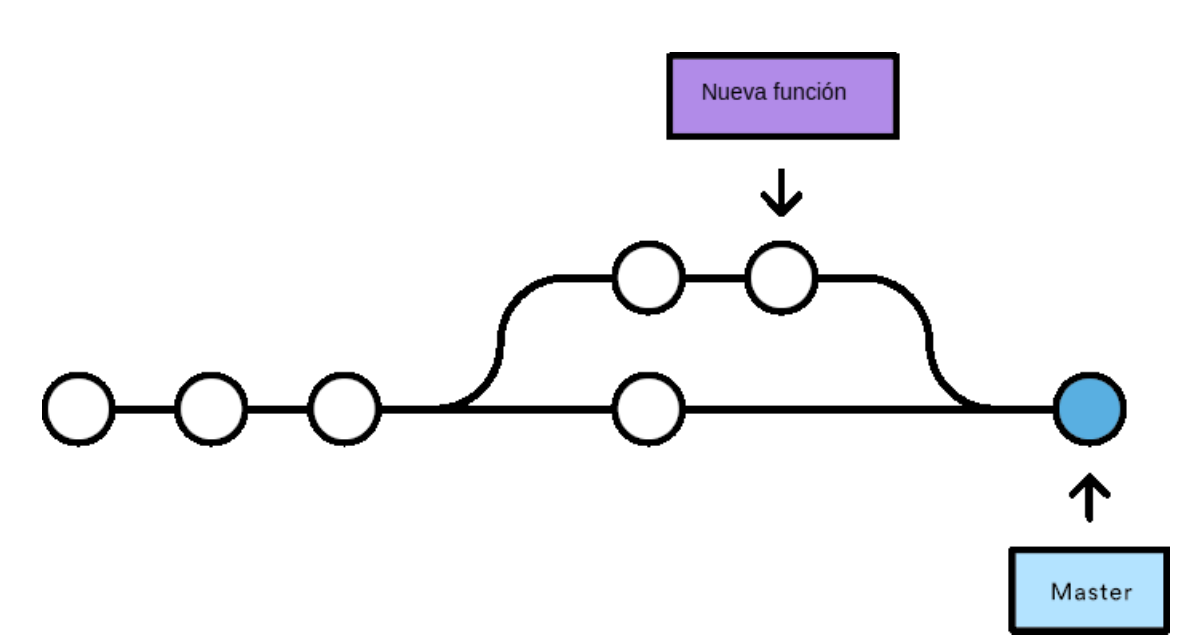
\includegraphics[width=\textwidth]{Resources/01.01.02-01.png}
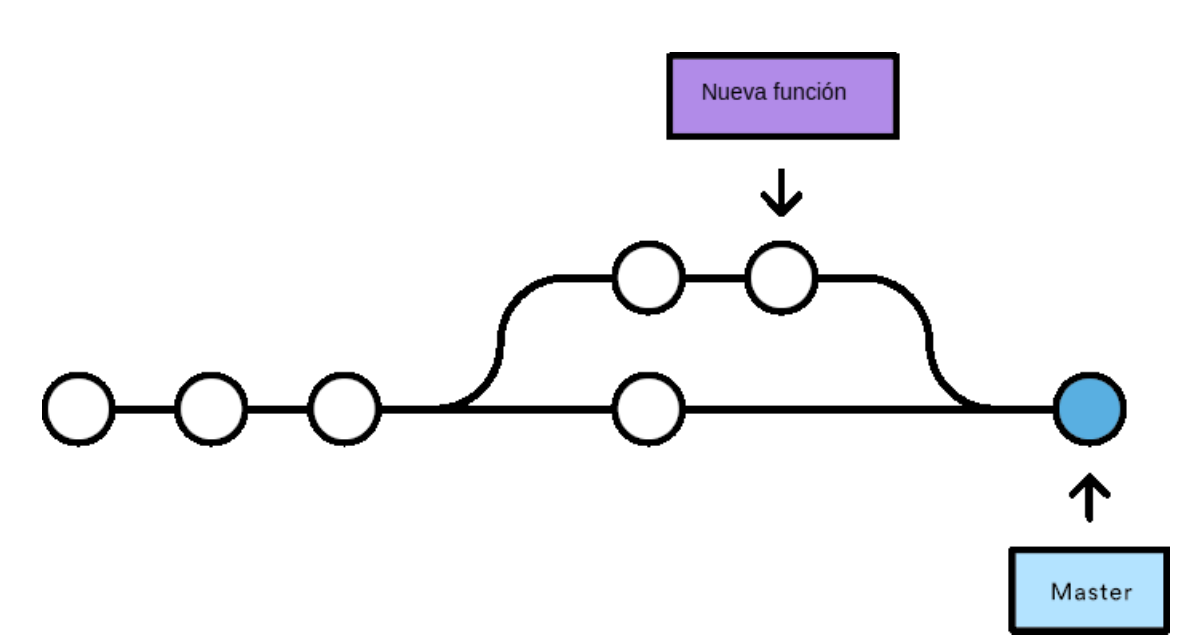
\includegraphics[width=0.95\textwidth]{Resources/01.01.02-01.png}

GitHub es una plataforma de desarrollo colaborativo que te permite alojar tus repositorios Git. Su uso es gratuito si el código almacenado es público. Además, te permite tener, una wiki y una página web para tu proyecto, junto a otras funciones.
Tanto el programa como este documento están disponibles en GitHub en el siguiente enlace. \url{https://github.com/daviddavo/InvProy}

\subsection{LaTeX}
\LaTeX\space o, en texto plano, LaTeX, pronunciado con la letra griega 
Ji ($\Chi$), es un software libre orientado a la creación de textos escritos comparable a la calidad tipográfica de las editoriales. Mediante la importación de paquetes y comandos o macros se puede dar formato al texto al igual que con cualquier otro editor, exportándolo posteriormente a PostScript o PDF. Está orientado a documentos técnicos y científicos por su facilidad a la hora de incluir fórmulas e importar paquetes que cumplan tus necesidades. No es un procesador de textos, pues está más enfocado en el contenido del documento que en la aparencia de éste.
El código del documento puede ser editado con cualquier editor de texto plano como \textit{nano} o \textit{emacs}, pero he usado una IDE llamada \textbf{texmaker}.

\subsection{Python}
Python es un lenguaje de programación interpretado (sólo traducen el programa a código máquina cuando se debe ejecutar esa parte del código, por lo que no hace falta compilarlo) que destaca por pretender una sintaxis más legible que la de el resto de lenguajes. Soporta tanto programación imperativo como programación orientada a objetos. Usa variables dinámicas, es multiplataforma, y, además, es de código abierto, lo que me permite distribuir el programa en Windows al distribuir los binarios de Python junto a él. En este caso, la versión de Python usada es la 3.4 en adelante.

\subsection{Gtk+}
Gtk+ es un conjunto de bibliotecas o \glspl{Libr} (conjunto de funciones y clases ya definidas preparadas para el uso de los programadores) desarrollado por la GNOME foundation destinado a la creación de GUIs (Interfaz Gráfica de Usuario), también, al igual que Linux forma parte del proyecto GNU.

Contiene las bibliotecas de GTK, GDK, ATK, Glib, Pango y Cairo; de las que he usado fundamentalmente GTK para crear la interfaz principal del programa; GDK al usarlo como intermediario entre los gráficos de bajo nivel y alto nivel y Cairo para la creación de algunos de los elementos gráficos del programa.

Al usar este conjunto de librerías, he conseguido que sólo sea necesario descargar una dependencia del programa, que además suele venir instalada en la mayoria de distros de Linux, por ejemplo en una instalación limpia de Ubuntu 16 (sin descargar paquetes adiccionales) el programa funciona perfectamente. Para usarlo en Linux se ha tenido que importar la libreria de PyGtk.
\subsection{Atom}
Atom es un editor de código multiplataforma con soporte para plugins escrito en Node.js, también tiene soporte para Git. También es un programa de código libre haciendo uso de la licencia MIT.

\subsection{Wireshark}
Wireshark es un \textit{packet sniffer} o analizador de paquetes. Te muestra los paquetes de red reales enviados y recibidos por una tarjeta de red, lo que facilita la creación del simulador de redes.

\chapter{Redes Informáticas}

\section*{Historia}
Internet, tal y como lo conocemos ahora, haciendo uso de IPv6, HTML5, CSS3 no existe hasta hace recientemente, pero el desarrollo de éste transcurre desde los años 60. En 1961 se publican los primeros artículos de \gls{conmutacion de paquetes}

\section{Capas de Red/Modelo OSI}
El modelo \acrshort{osi} es un modelo de referencia para redes basado en \gls{capas de abstraccion}
El objetivo del modelo \acrshort{osi} es conseguir la interoperabilidad entre sistemas con la protocolos estandarizados.

\definecolor{odd}{HTML}{FFFFFF}
\definecolor{even}{HTML}{E0E0E0}
\definecolor{header}{HTML}{42A5F5}

\rowcolors{2}{odd}{even}
\begin{tabular}{l|c|p{7cm}|p{2cm}}
	\hline
	\rowcolor{header}
	\textbf{Capa} & \textbf{PDU} & \textbf{Función} & \textbf{Ejemplos} \\
	1. Física & Bit & Transmisión y recepción de bits físicos sobre un medio físico & 	 RJ45, IEEE 802.11, etc. \\
	2. Data Link & Frame & Transmisión segura de \textit{frames} entre dos nodos conectados por una capa física. & Ethernet, 802.11, etc...\\
	3. Red & Paquete & Estructurar y administrar una red multinodo. Incluye enrutamiento, control de tráfico, y asignación de direcciones & IPv4, IPv6, ICMP... \\
	4. Transporte & \begin{tabular}[t]{@{}c@{}}Datagrama(UDP)\\Segmento(TCP)  \end{tabular} &
	Transmisión de segmentos de datos entre los puntos de una red, incluyendo ACK & TCP, UDP...\\
	5. Sesión &  & Administración de sesiones de comunicación, como intercambio continúo de información entre dos nodos. & SSH, RPC, PAP...\\ 
	6. Presentación & \multirow{3}{*}{Datos} & Translación de datos entre un servicio de red y una aplicación. Incluye comprensión, encriptación/decriptación, y codificación de carácteres. & MIME, TLS \\
	7. Aplicación & & APIs de alto nivel, incluyendo recursos compartidos y acceso remoto de archivos & HTTP, FTP, SMTP... \\ \hline
	
\end{tabular}

\glsaddall
\printglossaries

\newpage
\thispagestyle{empty}
\topskip0pt
\vspace*{\fill}
\doclicenseThis
\vspace*{\fill}
\end{document}
